\documentclass[tikz,border=10pt]{standalone}
\usepackage{tikz}
\usetikzlibrary{shapes.geometric, arrows.meta, positioning}

\tikzset{
    register/.style={
        rectangle, draw=black, thick,
        minimum width=1.5cm, minimum height=0.9cm,
        fill=white, font=\small\ttfamily
    },
    mux/.style={
        trapezium, trapezium left angle=70, trapezium right angle=110,
        draw=black, thick,
        minimum width=0.9cm, minimum height=0.75cm,
        fill=white, font=\small
    },
    alu/.style={
        rectangle, draw=black, thick,
        minimum width=1.1cm, minimum height=0.9cm,
        fill=white, font=\small
    },
    wire/.style={draw=black, thick, -Stealth},
    bus/.style={draw=black, line width=1.5pt, -Stealth},
    controlwire/.style={draw=black!60, dashed, -Stealth},
    buswidth/.style={font=\tiny, fill=white, inner sep=1pt},
    logic/.style={
        rectangle, draw=black, thick, rounded corners=3pt,
        minimum width=0.9cm, minimum height=0.75cm,
        fill=gray!10, font=\small
    },
    sbox/.style={
        rectangle, draw=black, thick,
        minimum width=0.75cm, minimum height=0.75cm,
        fill=gray!20, font=\small
    }
}

\begin{document}
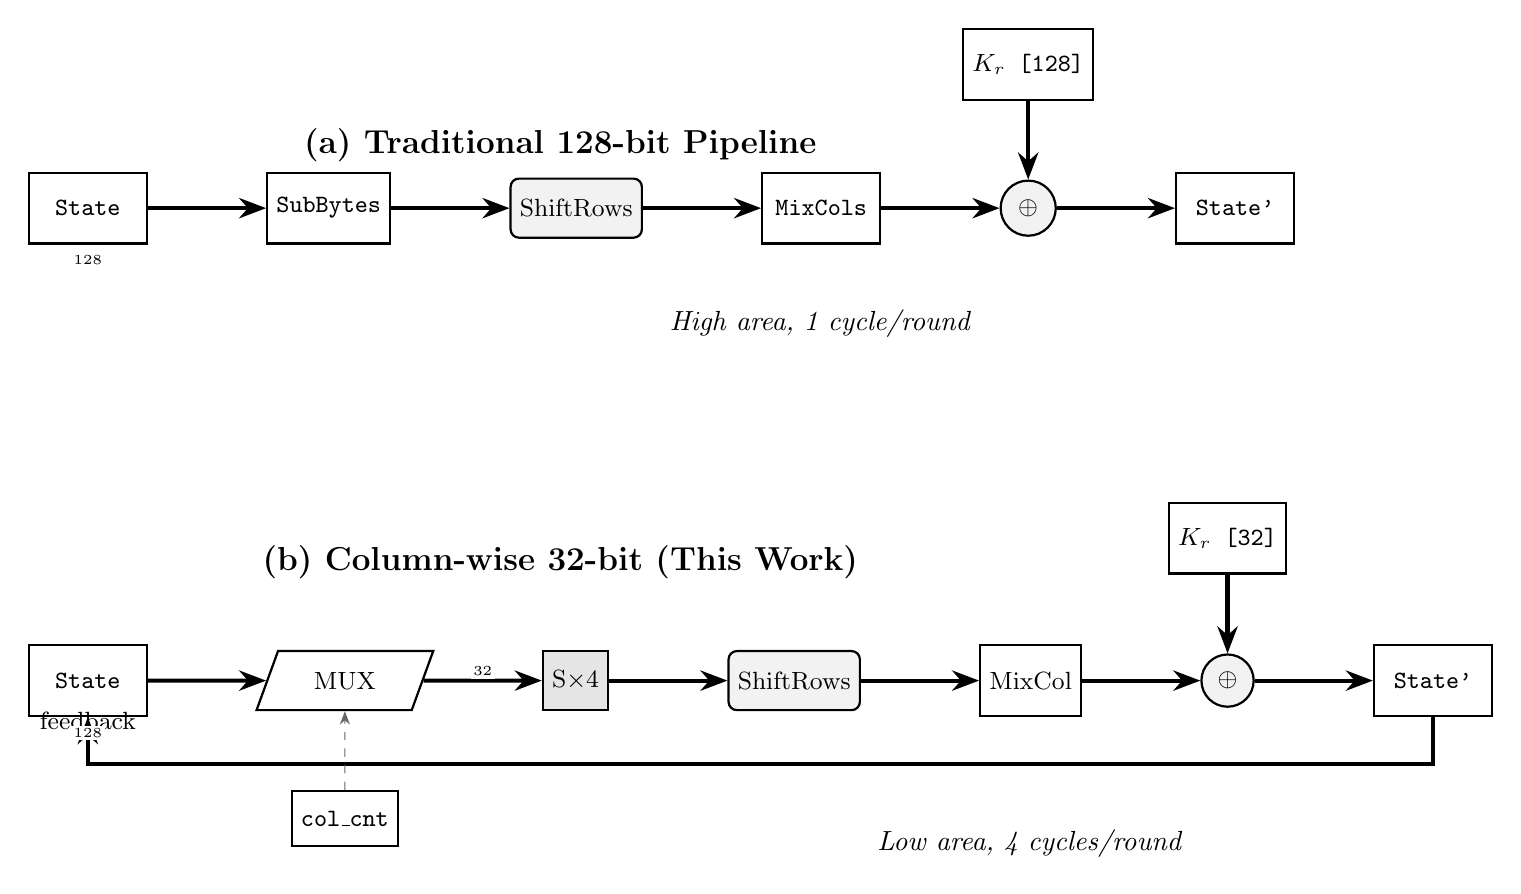
\begin{tikzpicture}[node distance=1.2cm and 1.5cm]

% (a) Traditional 128-bit Pipeline
\node[font=\large\bfseries] at (6,0.8) {(a) Traditional 128-bit Pipeline};

\node[register] (s0) at (0,0) {State};
\node[register, right=of s0] (sb) {SubBytes};
\node[logic, right=of sb] (sr) {ShiftRows};
\node[register, right=of sr] (mc) {MixCols};
\node[logic, circle, minimum size=0.7cm, right=of mc] (xor) {$\oplus$};
\node[register, right=of xor] (s1) {State'};

\node[register, above=1cm of xor] (rk) {$K_r$ [128]};

\draw[bus] (s0) -- (sb);
\draw[bus] (sb) -- (sr);
\draw[bus] (sr) -- (mc);
\draw[bus] (mc) -- (xor);
\draw[bus] (xor) -- (s1);
\draw[bus] (rk) -- (xor);

\node[buswidth, below=0.1cm of s0.south] {128};
\node[font=\normalsize, below=0.7cm of mc] {\textit{High area, 1 cycle/round}};

% (b) Column-wise 32-bit Pipeline
\node[font=\large\bfseries] at (6,-4.5) {(b) Column-wise 32-bit (This Work)};

\node[register] (t0) at (0,-6) {State};
\node[mux, right=of t0] (tmux) {MUX};
\node[sbox, right=of tmux] (tsb) {S$\times$4};
\node[logic, right=of tsb, minimum width=1.3cm] (tsr) {ShiftRows};
\node[alu, right=of tsr] (tmc) {MixCol};
\node[logic, circle, minimum size=0.65cm, right=of tmc] (txor) {$\oplus$};
\node[register, right=of txor] (t1) {State'};

\node[register, above=1cm of txor, minimum width=1.3cm] (trk) {$K_r$ [32]};
\node[register, below=1cm of tmux, minimum width=1.1cm, minimum height=0.7cm] (cnt) {col\_cnt};

\draw[bus] (t0) -- (tmux);
\draw[bus] (tmux) -- node[buswidth, above] {32} (tsb);
\draw[bus] (tsb) -- (tsr);
\draw[bus] (tsr) -- (tmc);
\draw[bus] (tmc) -- (txor);
\draw[bus] (txor) -- (t1);
\draw[bus] (trk) -- (txor);
\draw[bus] (t1.south) -- ++(0,-0.6) -| node[near end, above, font=\small] {feedback} (t0.south);
\draw[controlwire] (cnt) -- (tmux);

\node[buswidth, below=0.1cm of t0.south] {128};
\node[font=\normalsize, below=1.3cm of tmc] {\textit{Low area, 4 cycles/round}};

\end{tikzpicture}
\end{document}
